\section{Introduction} \label{sec: introduction}


\begin{figure}[!t]
  \centering
  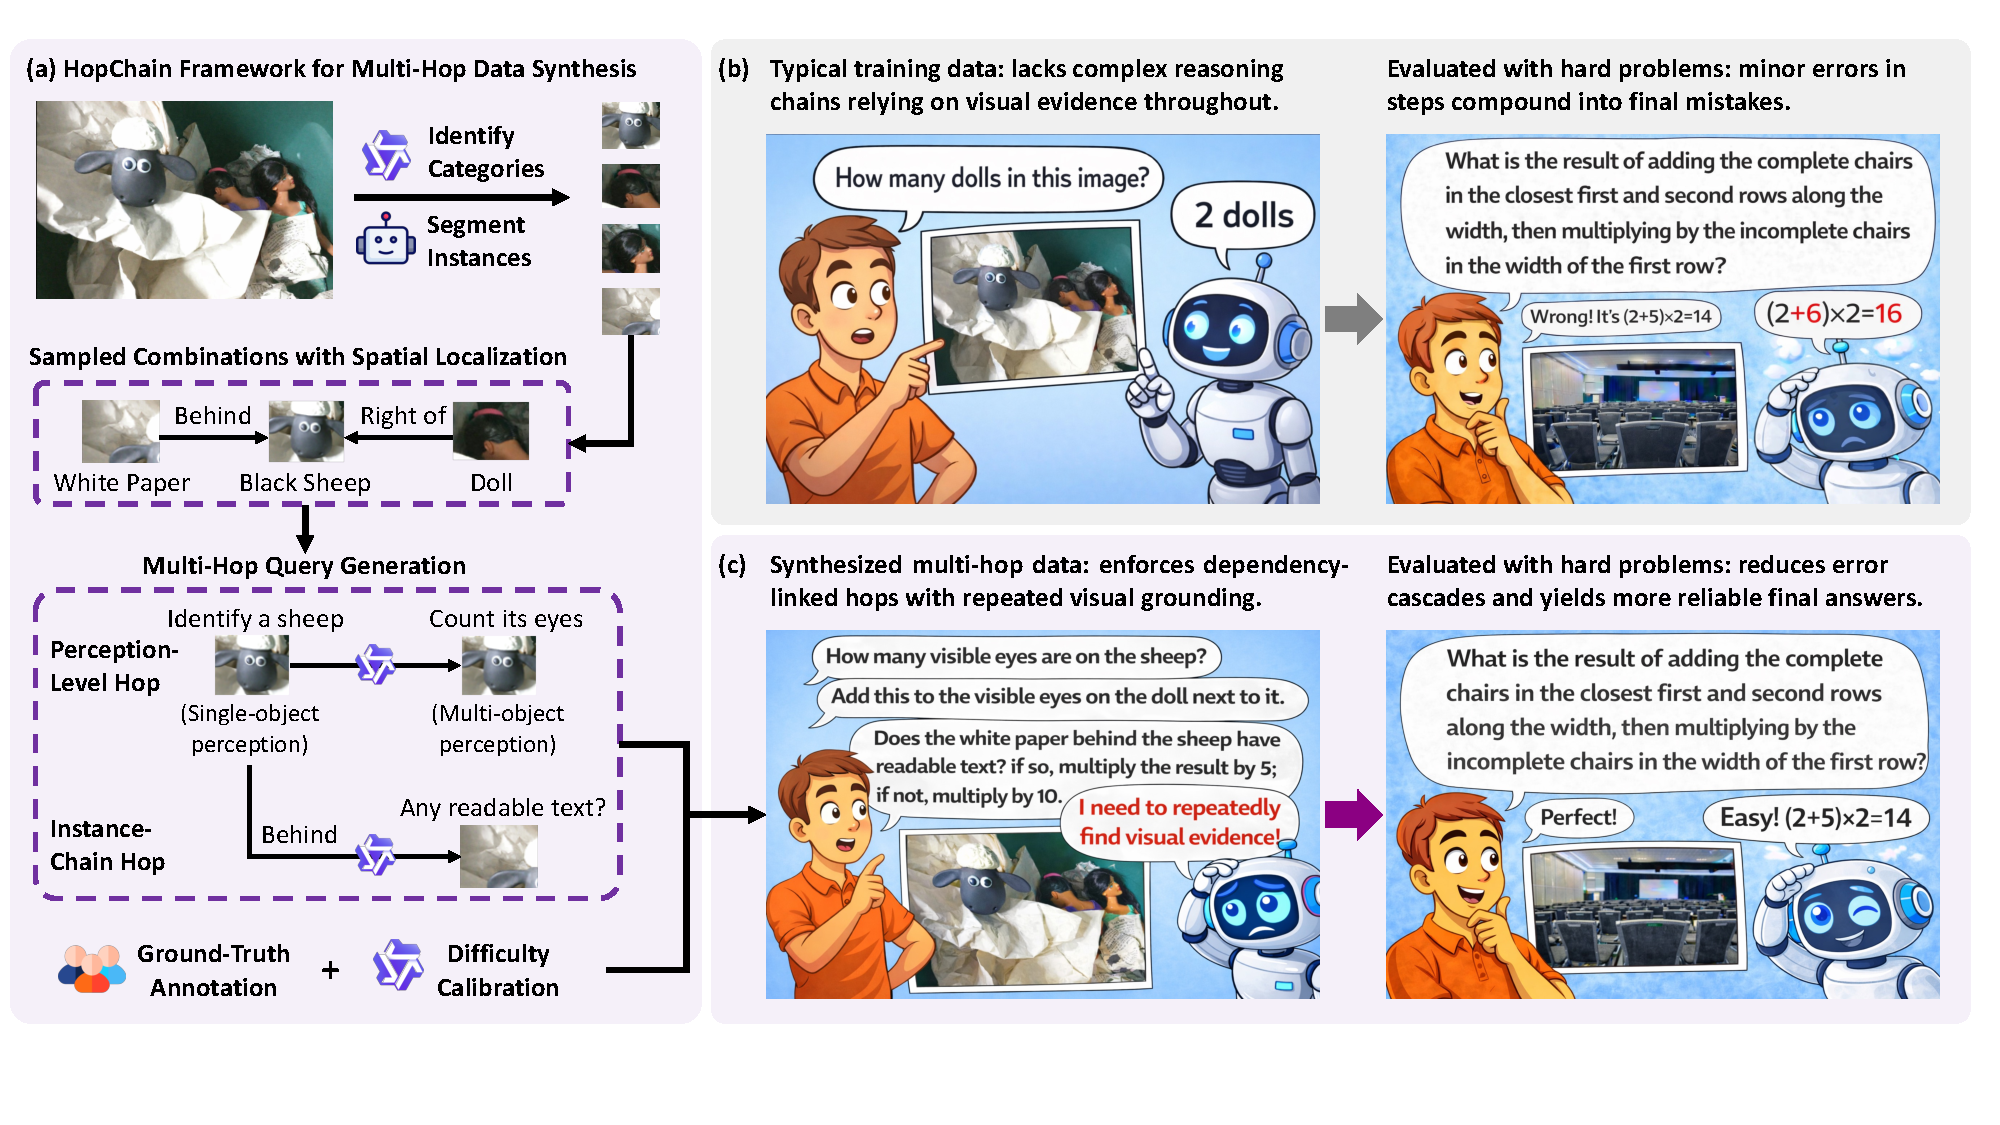
\includegraphics[width=1\textwidth]{imgs/teaser_multihop_4.pdf}
  \caption{Overview of HopChain and the motivation for multi-hop vision-language reasoning data. \textbf{(a)} HopChain synthesizes multi-hop data through four stages: category identification, instance segmentation, multi-hop query generation, and ground-truth annotation with difficulty calibration. \textbf{(b)} Typical vision-language training data often does not require complex reasoning chains that rely on visual evidence throughout; on hard problems, minor mistakes introduced at intermediate long-CoT steps can compound into final errors. \textbf{(c)} In contrast, the multi-hop data synthesized by HopChain forms logically dependent hop chains in which later hops depend on instances, sets, or conditions established by earlier hops, while nearly every hop requires fresh visual re-grounding. This training signal encourages continual visual evidence seeking during long-CoT reasoning, improving robustness and reducing compounding errors.}
  \label{fig:example_image}
  \vspace{-6pt}
\end{figure}

Vision-language models (VLMs) have achieved impressive performance across a diverse set of multimodal benchmarks by integrating visual encoders with large language models~\CiteParen{liu2024visual,liu2024improved,bai2023qwenvl,bai2025qwen25vl,chen2024internvl,openai2023gpt4,geminiteam2024gemini}.
Recent advances in reinforcement learning with verifiable rewards (RLVR) have further improved VLMs' reasoning abilities by training them to produce step-by-step chain-of-thought solutions for questions with objectively verifiable answers~\CiteParen{shao2024deepseekmath,deepseekr1}.
Despite this progress, a critical gap remains: VLMs frequently struggle with tasks that require \emph{fine-grained, multi-step vision-language reasoning}, where the correct answer depends on carefully attending to multiple visual elements and their relationships within an image~\CiteParen{bigverdi2025perception,ye2025blinktwice,jiang2025vlmr3}.


A natural question arises: \emph{what prevents current VLMs from performing robust vision-language reasoning?}
In \cref{sec: unreliable visual perception in long-chain reasoning}, we analyze a central challenge:
VLMs exhibit \textbf{diverse and compounding failure modes during long chain-of-thought (CoT) reasoning}, as longer reasoning chains may cause models to attend less faithfully to the image, execute incorrect intermediate reasoning steps, rely on incomplete knowledge, or produce hallucinated and weakly grounded intermediate content that then compounds across subsequent steps.
Related failure patterns have also been reported in prior analyses of amplified multimodal hallucination, evidential drift, object hallucination, visual illusion, and image-context reasoning errors~\CiteParen{liu2025morethinking,luo2025thinkingdrifts,rohrbach2018object,guan2024hallusionbench,leng2024vcd}.
Critically, as depicted in \cref{fig:example_image}(b), most existing vision-language training data does not involve particularly complex reasoning chains that depend on visual evidence throughout the process.
As a result, these long-CoT weaknesses remain largely unexposed during training.
This observation suggests that relying on, or simply expanding, existing vision-language RLVR training data is insufficient; what is needed is training data that \emph{structurally forces} the model to seek visual evidence at each step of long-CoT reasoning, strengthening step-by-step vision-language reasoning and improving generalization across diverse scenarios.


Motivated by this insight, we propose \textbf{HopChain}\footnote{Throughout this paper, HopChain refers to our synthesis framework, while \emph{multi-hop vision-language reasoning data}, or simply \emph{multi-hop data}, refers to the training data synthesized by HopChain.}, a scalable framework for synthesizing multi-hop vision-language reasoning data specifically for RLVR training of VLMs.
Each synthesized multi-hop query forms a logically dependent chain of instance-grounded hops, where earlier hops establish the instances, sets, or conditions needed for later hops, forcing repeated visual re-grounding throughout training rather than language-only shortcuts.
At the same time, each query terminates in a specific, unambiguous numerical answer that is easy to verify for RLVR; moreover, because the hops are logically dependent, obtaining the correct final number usually also requires the intermediate reasoning steps to be correct.
Rather than targeting a narrow synthetic task, we use the multi-hop data synthesized by HopChain as a complementary source of RLVR training data to strengthen fundamental vision-language reasoning under long CoT and support broad, generalizable gains across diverse domains.
Importantly, this synthesized data is not tailored to any particular downstream benchmark; instead, it is constructed to strengthen general-purpose vision-language reasoning, which we later show transfers broadly across benchmark families.
We define this multi-hop structure through two hop types: perception-level hops and instance-chain hops.
A \emph{perception-level hop} switches between single-object perception (e.g., read text, identify color, determine position) and multi-object relationship reasoning (e.g., compare sizes, count objects satisfying a condition, determine spatial arrangement), while remaining grounded in the instances, sets, or conditions established by earlier hops.
An \emph{instance-chain hop} follows an explicit dependency chain (e.g., instance A $\rightarrow$ B $\rightarrow$ C), where the next instance can be identified only from the instances, sets, or conditions established by earlier hops.
We require each query to combine both hop types in a logically dependent chain, where earlier hops establish the instances, sets, or conditions needed for later hops.
This design forces fresh visual grounding at every step, blocks language-only shortcuts, and exposes diverse long-CoT failure modes during training, as shown in \cref{fig:example_image}(c).

To construct such multi-hop data at scale, HopChain adopts a scalable four-stage data synthesis pipeline:
(1)~\emph{category identification} via Qwen3-VL-235B-A22B-Thinking~\CiteParen{qwen3vl2025} to enumerate semantic categories in each image;
(2)~\emph{instance segmentation} via SAM3~\CiteParen{carion2025sam3} to localize individual instances for the identified semantic categories;
(3)~\emph{multi-hop query generation} via Qwen3-VL-235B-A22B-Thinking that constructs logically chained questions over combinations of instances; and
(4)~\emph{human-in-the-loop verification} where multiple annotators independently solve each query, and only queries with the same final numerical answer are retained as valid training examples.
The pipeline provides a scalable data synthesis workflow, scaling to broad image collections with sufficient detectable instances while maintaining strict quality control, as summarized in \cref{fig:example_image}(a).

We apply RLVR with Soft Adaptive Policy Optimization (SAPO)~\CiteParen{sapo} on the multi-hop data synthesized by HopChain to train VLMs.
We validate the effectiveness of the multi-hop data synthesized by HopChain on Qwen3.5-35B-A3B and Qwen3.5-397B-A17B~\CiteParen{qwen35blog} across 24 benchmarks spanning STEM and Puzzle, General VQA, Text Recognition and Document Understanding, and Video Understanding.
Compared with RLVR on the original RLVR data alone, adding this multi-hop data improves 20 out of 24 benchmarks on both Qwen3.5-35B-A3B and Qwen3.5-397B-A17B, despite the fact that the synthesized data is not designed for any specific benchmark, indicating broad and generalizable performance gains across diverse scenarios.
To demonstrate that full chained queries are important, we replace them with half-multi-hop or single-hop variants on Qwen3.5-35B-A3B, reducing the average score across five representative benchmarks from 70.4 to 66.7 and 64.3, respectively.
Multi-hop training substantially strengthens long-CoT vision-language reasoning, with gains peaking at more than 50 accuracy points in the ultra-long-CoT regime on Qwen3.5-397B-A17B.
When we independently sample each synthesized query multiple times on both Qwen3.5-35B-A3B and Qwen3.5-397B-A17B, more than half of the queries are partially solved and the outcomes are distributed relatively evenly from fully incorrect to fully correct, indicating a broad difficulty range suitable for both smaller and larger models. The corrected error types also closely follow the original error distribution before adding this multi-hop data, indicating gains that are broad rather than confined to a single narrow failure mode.
These extensive experiments establish HopChain as an effective framework for synthesizing multi-hop data that improves generalizable vision-language reasoning capabilities beyond the synthesized training distribution.

\vspace{0.3em}
\noindent Our main contributions are as follows:
\begin{itemize}[leftmargin=1.5em, itemsep=2pt, topsep=2pt]
    \item We identify diverse and compounding failure modes during long CoT reasoning as a key barrier to vision-language generalization, and show why relying on or simply expanding existing vision-language RLVR training data is insufficient.
    \item We formalize multi-hop vision-language reasoning with perception-level and instance-chain hops, and build HopChain, a scalable synthesis pipeline whose queries form logically dependent chains in which earlier hops establish the instances, sets, or conditions needed for later hops, forcing repeated visual re-grounding throughout training while keeping the final answer directly verifiable for RLVR.
    \item Through extensive experiments, we verify that RLVR on the multi-hop data synthesized by HopChain yields broad, generalizable gains: 20 out of 24 benchmarks improve on both Qwen3.5-35B-A3B and Qwen3.5-397B-A17B, while additional analyses show that preserving full chained queries is important, multi-hop data strengthens long-CoT vision-language reasoning, and the synthesized data spans a broad difficulty range while enabling trained models to correct a broad range of errors.
\end{itemize}
